\documentclass[11pt,a4paper]{article}

% ============================================================
% Comprobante de Registro OSF — CarniCore — Entrega 3 (2A)
% ISR-401 / 20303 — UTEQ
% Versión 2.0 — corrige el identificador OSF citado (ver Erratum)
% ============================================================

\usepackage[utf8]{inputenc}
\usepackage[T1]{fontenc}
% Si el sistema tiene instalado texlive-lang-spanish, se puede activar:
% \usepackage[spanish]{babel}
\usepackage{geometry}
\geometry{a4paper, margin=2.5cm}
\usepackage{longtable}
\usepackage{booktabs}
\usepackage{array}
\usepackage{colortbl}
\usepackage{xcolor}
\usepackage{graphicx}
\usepackage{hyperref}
\usepackage{enumitem}
\usepackage{titlesec}
\usepackage{fancyhdr}
\usepackage{tabularx}
\usepackage{float}
\usepackage{framed}

% -------------------- Colores institucionales --------------------
\definecolor{uteqverde}{RGB}{0,90,60}
\definecolor{griscelda}{RGB}{240,240,240}
\definecolor{alerta}{RGB}{140,20,20}

% -------------------- Encabezado y pie de página --------------------
\pagestyle{fancy}
\fancyhf{}
\renewcommand{\headrulewidth}{0.6pt}
\renewcommand{\footrulewidth}{0.4pt}
\lhead{\small UTEQ -- Ingeniería de Requerimientos (ISR-401 / 20303)}
\rhead{\small Comprobante de Registro OSF -- CarniCore -- Entrega 3 (2A)}
\cfoot{\thepage}

\hypersetup{
    colorlinks=true,
    linkcolor=uteqverde,
    urlcolor=uteqverde,
    citecolor=uteqverde,
    pdftitle={Comprobante de Registro OSF -- CarniCore -- Entrega 3 (2A) -- v2.0},
    pdfauthor={Equipo CarniCore -- UTEQ ISR-401},
}

\titleformat{\section}
  {\normalfont\Large\bfseries\color{uteqverde}}{\thesection}{1em}{}
\titleformat{\subsection}
  {\normalfont\large\bfseries}{\thesubsection}{1em}{}

% -------------------- Entornos de nota --------------------
\newenvironment{notacumplimiento}
  {\begin{framed}\small\noindent\textbf{Nota de cumplimiento.}~}
  {\end{framed}}

\newenvironment{notaerratum}
  {\begin{framed}\small\noindent\textbf{\color{alerta}Erratum (corrige la v1.0 de este documento).}~}
  {\end{framed}}

\begin{document}

% ============================================================
% PORTADA / TÍTULO
% ============================================================
\begin{center}
    {\Large\bfseries Comprobante de Registro Previo en OSF}\\[0.3em]
    {\large Componente Empírico -- Sistema CarniCore -- Enfoque 2}\\[0.6em]
    {\small Ubicación en el repositorio: \texttt{06\_Experimento/osf\_registration.pdf}}
\end{center}

\vspace{0.5em}
\hrule
\vspace{1em}

% ============================================================
% ERRATUM
% ============================================================
\begin{notaerratum}
La versión 1.0 de este documento identificaba el registro con el enlace
\url{https://osf.io/wud69}. Ese identificador corresponde al \textbf{proyecto} de
OSF, de visibilidad \textbf{privada}, no al \textbf{registro} (\textit{registration})
propiamente dicho. \texttt{README.md} y \texttt{CHANGELOG.md} ya documentaban esta
corrección --el identificador correcto del registro es \url{https://osf.io/yp7t3},
público desde su creación-- y la propagaron a los demás archivos del repositorio,
pero este documento, que es precisamente el comprobante, había quedado sin corregir.
Esta versión 2.0 lo corrige y ajusta los campos que dependían del objeto equivocado.
\end{notaerratum}

% ============================================================
% DATOS DEL REGISTRO
% ============================================================
\section*{Datos del registro}

\renewcommand{\arraystretch}{1.4}
\begin{longtable}{@{}>{\bfseries}p{4.2cm} p{10.8cm}@{}}
\toprule
\rowcolor{griscelda}
Campo & Valor \\
\midrule
\endhead

Enlace del registro & \url{https://osf.io/yp7t3} \\
Naturaleza del objeto & \textit{Registration} pública de OSF (no el proyecto
\texttt{osf.io/wud69}, que es privado y no constituye por sí mismo comprobante
verificable por un tercero) \\
Fecha de creación (\textit{Date Created}) &
02 de agosto de 2026, 12:31~PM \textit{(leída directamente del sello que OSF
muestra en la página del registro \texttt{yp7t3})} \\
Fecha de registro (\textit{Date registered}) &
02 de agosto de 2026, 12:31~PM \textit{(idéntica a la fecha de creación: OSF
registra que este objeto se creó y se registró en el mismo acto, sin período de
borrador previo; leída directamente de la página del registro \texttt{yp7t3})} \\
Título del registro &
Detección automática de ambigüedad en requisitos funcionales: un estudio de caso
en el dominio de trazabilidad cárnica (CarniCore) \\
Visibilidad & Pública (\textit{Public registration}) --- verificable por
cualquier persona con el enlace, sin necesidad de sesión autenticada \\
Plantilla y registro &
\textit{Registration Type:} OSF Preregistration; \textit{Registry:} OSF
Registries \textit{(visibles en el panel lateral del Overview, Figura~\ref{fig:osf-overview})} \\
Licencia & CC0 1.0 Universal \textit{(confirmada en el panel lateral del
registro \texttt{yp7t3})} \\
DOI del registro &
\href{https://doi.org/10.17605/OSF.IO/YP7T3}{10.17605/OSF.IO/YP7T3} ---
\textit{a diferencia de la v1.0, que reportaba ``sin DOI'' (dato correcto para
el proyecto \texttt{wud69}, pero no aplicable al registro), el registro
\texttt{yp7t3} sí tiene DOI propio asignado} \\
Copia de respaldo independiente &
\url{https://archive.org/details/osf-registrations-yp7t3-v1} --- snapshot del
registro en Internet Archive, con sello de fecha propio y ajeno tanto al
equipo como a OSF; constituye una segunda fuente de verificación externa,
independiente de las capturas de pantalla \\
Protocolo adjunto &
\texttt{protocolo.pdf} (versión 1.0, 02/08/2026), consistente con el contenido del
formulario de registro \\
\bottomrule
\end{longtable}

% ============================================================
% VERIFICACIÓN DE PRECEDENCIA TEMPORAL
% ============================================================
\section*{Verificación de precedencia temporal}

Conforme al gatekeeper G6 de la Guía y Rúbrica de la Entrega 3 (2A), el registro debe
tener fecha anterior a toda recolección de datos (envío de la primera ficha de
clasificación experta y ejecución del detector).

El registro \url{https://osf.io/yp7t3} tiene fecha de creación y de registro
coincidentes: 02/08/2026, 12:31~PM (ambos sellos, \textit{Date Created} y
\textit{Date registered}, leídos directamente de la página del registro). Esa
fecha es anterior a la ejecución del análisis y del panel experto del componente
empírico, que el equipo inicia únicamente después de este registro, conforme al
procedimiento de la Sección 8 del protocolo.

A diferencia del objeto \texttt{wud69} (privado, solo verificable con capturas
tomadas por el propio equipo), \textbf{\texttt{yp7t3} es un registro público}: el
sello de fecha que OSF le asigna es visible y verificable por cualquier tercero
--incluido el tribunal evaluador-- visitando el enlace directamente, sin depender de
una captura de pantalla del equipo. Esa verificabilidad independiente es, en
sentido estricto, lo que convierte el enlace en comprobante y no en un simple
indicio.

El propio formulario de registro declara explícitamente, en el campo
\textit{Foreknowledge of data or evidence}:

\begin{quote}
\itshape
``Data does not yet exist. No part of the data that will be used for this analysis
plan exists, and no part will be generated until after this plan is registered.''
\end{quote}

Esta declaración, hecha por el equipo al momento de registrar, constituye evidencia
adicional de precedencia temporal.

% ============================================================
% CONSISTENCIA CON EL PROTOCOLO
% ============================================================
\section*{Consistencia con el protocolo}

Se verificó que el contenido del formulario de registro (preguntas de investigación,
hipótesis H0/H1, diseño censal sobre 25 RF, cegamiento y aleatorización con semilla
fija, métricas de precisión/\textit{recall}/F1/$\kappa$ de Cohen y Fleiss, software en
Python) es consistente con las Secciones 3, 4, 6, 9 y 10 de \texttt{protocolo.pdf}
versión 1.0. No se detectaron contradicciones entre ambos documentos.

% ============================================================
% CAPTURAS DE PANTALLA
% ============================================================
\section*{Capturas de pantalla}

\begin{notaerratum}
La v1.0 de este documento describía ambas capturas como pertenecientes al
proyecto privado \texttt{wud69}. Revisando el contenido real de las imágenes,
eso solo es cierto para la primera: es un recorte del campo \textit{Associated
Project} del panel lateral del propio registro \texttt{yp7t3}, que indica que
su proyecto de origen (\texttt{osf.io/wud69}) es privado -- un dato normal y
esperado, no un error: en OSF una \textit{registration} puede tener un
proyecto de origen privado sin que eso afecte la visibilidad pública del
registro en sí. La segunda captura es en realidad el \textbf{Overview del
propio registro} \texttt{yp7t3} (pestaña \textit{Registry Details ->
Overview}), no del proyecto: muestra el contenido íntegro del preregistro y,
en su panel lateral, \textit{Registration Type: OSF Preregistration},
\textit{Registry: OSF Registries} y los sellos \textit{Date Created} /
\textit{Date Registered} -- exactamente los que se citan en la tabla de esta
página. Se corrigen aquí las leyendas de ambas figuras.
\end{notaerratum}

\begin{figure}[H]
    \centering
    \includegraphics[width=0.6\textwidth]{figures/osf_proyecto_asociado.png}
    \caption{Campo \textit{Associated Project} del panel lateral del registro
    \texttt{osf.io/yp7t3}, mostrando que su proyecto de origen
    (\texttt{osf.io/wud69}) es privado.}
\end{figure}

\begin{figure}[H]
    \centering
    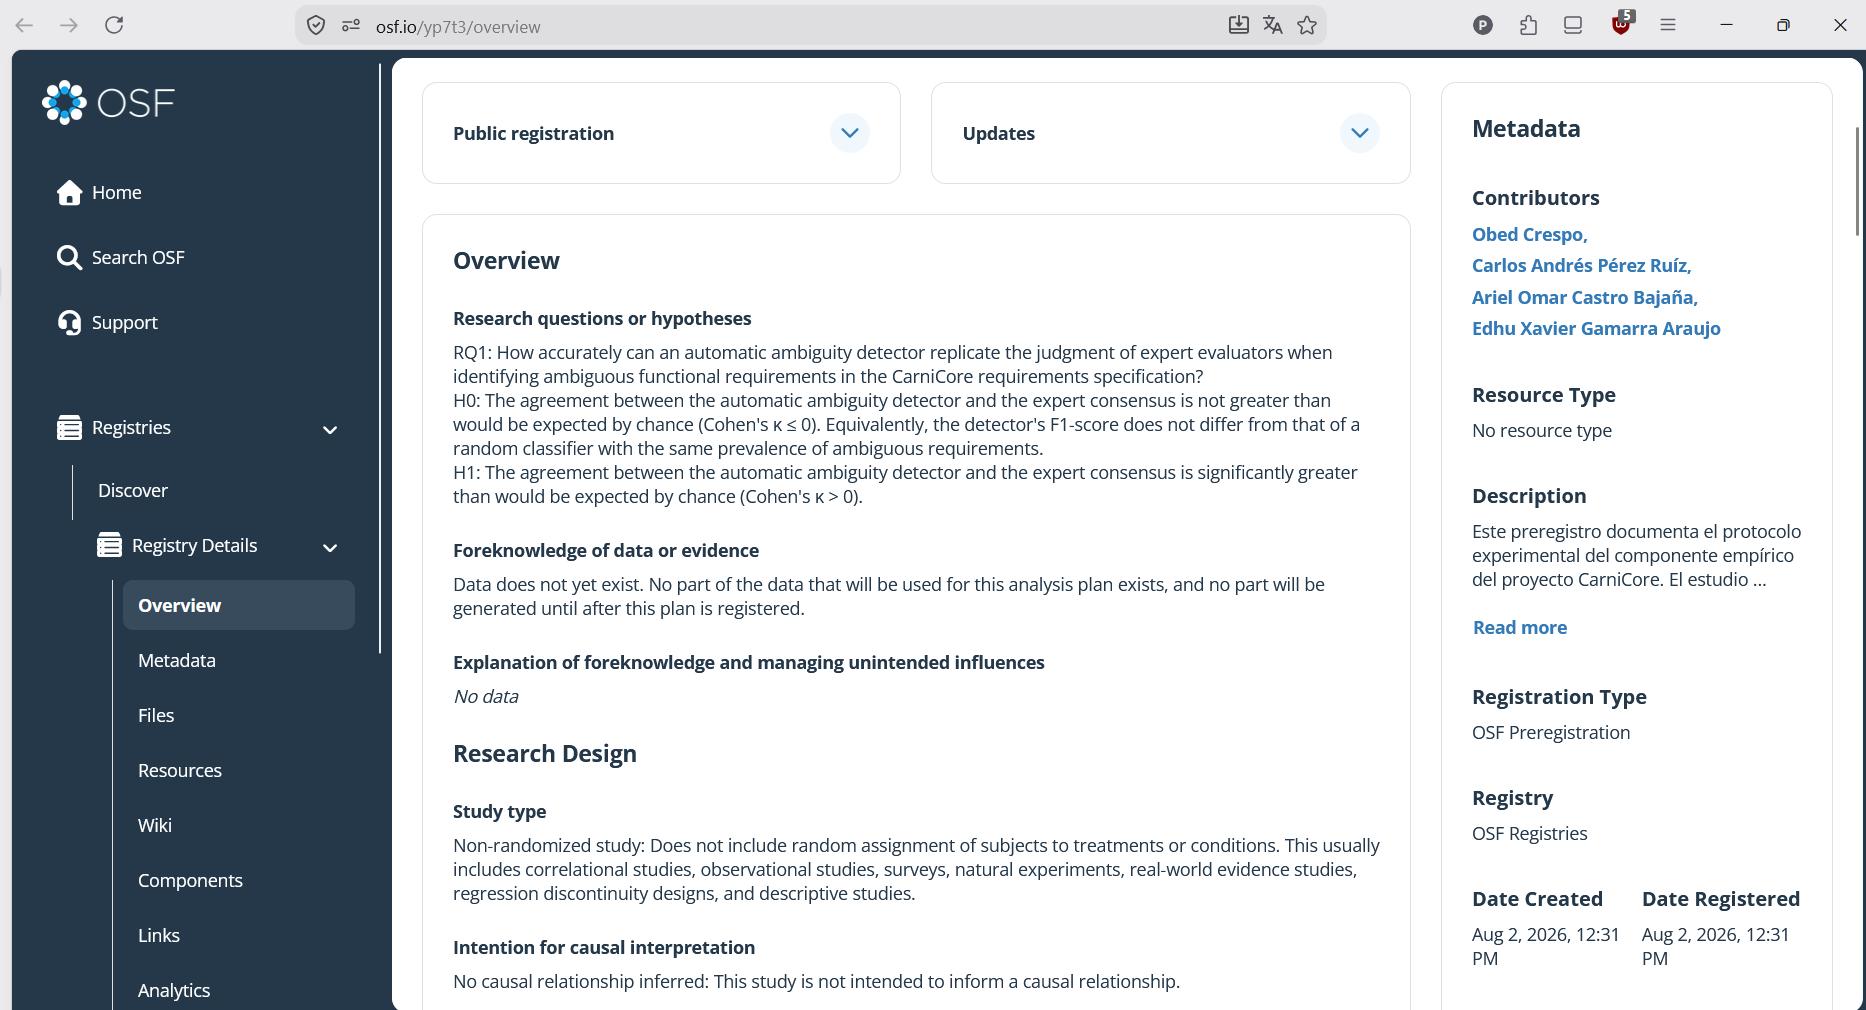
\includegraphics[width=\textwidth]{figures/osf_detalle_registro.png}
    \caption{Overview del registro \texttt{osf.io/yp7t3} en OSF, con la barra
    de direcciones del navegador visible (\texttt{osf.io/yp7t3/overview}):
    contenido del preregistro (preguntas de investigación, H0/H1,
    \textit{Foreknowledge of data}, diseño de la investigación), autores, y
    panel lateral con \textit{Registration Type: OSF Preregistration} y los
    sellos \textit{Date Created} / \textit{Date Registered}: 2 de agosto de
    2026, 12:31~PM.}
    \label{fig:osf-overview}
\end{figure}

\begin{notacumplimiento}
Esta captura incluye, en una sola imagen, los tres elementos que exige el
comprobante: la barra de direcciones del navegador con la URL
\texttt{osf.io/yp7t3/overview}, el contenido del registro, y el sello
\textit{Date Registered} que asigna OSF. Al ser generada por la propia interfaz
de OSF -no redactada por el equipo- y mostrar una URL de un registro público,
es verificable de forma independiente por cualquier tercero que visite ese
enlace. Con esto queda cerrado el punto señalado sobre el comprobante externo
con sello temporal.
\end{notacumplimiento}

\vspace{1em}
\begin{notacumplimiento}
Este comprobante documenta únicamente los datos confirmados directamente por el
equipo contra el objeto correcto de OSF (\texttt{yp7t3}). Los campos que aún no se
han releído sobre ese objeto se marcan explícitamente como pendientes en la tabla
anterior; no se completa ningún campo por inferencia ni se reutilizan valores del
objeto \texttt{wud69}.
\end{notacumplimiento}

\end{document}
